\subsection{What You Should Know}

\begin{frame}{\myframetitle{}}
	\begin{mycolumns}
		\mynote{Fundamentals of Software Engineering}{
			\begin{itemize}
				\item development processes
				\item object-oriented programming
				\item design patterns
				\item UML class diagrams
				\item modularity
			\end{itemize}
			\ifuniversity{magdeburg}{$\Rightarrow$ \emph{Software Engineering}}
		}
	\mynextcolumn
		\mynote{Fundamentals of Theoretical Computer Science}{
			\begin{itemize}
				\item set theory
				\item propositional logic
				\item complexity theory
			\end{itemize}
			\ifuniversity{magdeburg}{
				$\Rightarrow$ \emph{Logik}\\
				$\Rightarrow$ \emph{Grundlagen der Theoretischen Informatik I}
			}
		}

		\mynote{Exercise}{
			solid programming skills in Java

			\ifuniversity{magdeburg}{
				$\Rightarrow$ \emph{Einführung in die Informatik}\\
				$\Rightarrow$ \emph{Algorithmen und Datenstrukturen}
			}
		}
	\end{mycolumns}
\end{frame}

\subsection{What You Will Learn}

\begin{frame}{\myframetitle{}}
	\lectureseriesoverview
\end{frame}

\subsection{What You Might Need}

\begin{frame}{\myframetitle{}}
	\begin{mycolumns}
		\myexampletight{Recommended Literature for Lecture \& Exercise}{
			\centering
			\parbox{0.49\linewidth}{
				\centering
				\pic[width=\linewidth]{cover-fospl}
				\emph{theory-focused}
			}
			\parbox{0.475\linewidth}{
				\centering
				\pic[width=\linewidth]{cover-featureide}
				\emph{practice-oriented}
			}
		}
	\mynextcolumn
		\myexampletight{Recommended Tool Support for the Exercise}{
			\centering
			\pic[width=\linewidth]{featureide-feature-model-editor}\\[.5ex]
			\pic[width=0.25\linewidth]{featureide-logo}
		}
	\end{mycolumns}
\end{frame}

\subsection{Credit for the Slides}

\begin{frame}{\myframetitle{}}
	\vspace{-10mm}\hfill\href{https://github.com/SoftVarE-Group/Course-on-Software-Product-Lines}{
\includegraphics[scale=.5]{cc-by-sa}}\vspace{2mm}
	\begin{mycolumns}[columns=3,animation=none]
		\mynote{Thomas Thüm}{
			\centering
			\href{https://www.uni-ulm.de/en/in/sp/team/thuem/}{\adjincludegraphics[height=.45\textheight,trim={.125\width} 0 {.125\width} 0,clip]{thomas-thuem}}

			\small Professor at University of Ulm

			software engineering

			FeatureIDE team leader
		}
	\mynextcolumn
		\mynote{Timo Kehrer}{
			\centering
			\href{https://seg.inf.unibe.ch/people/timo/}{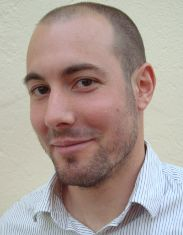
\includegraphics[height=.45\textheight]{timo-kehrer}}

			\small Professor at University of Bern

			software engineering

			~
		}
	\mynextcolumn
		\mynote{Elias Kuiter}{
			\centering
			\href{https://www.dbse.ovgu.de/en/Staff/Elias+Kuiter.html}{
\includegraphics[height=.45\textheight]{elias-kuiter}}

			\small PhD student in Magdeburg

			feature-model analysis

			FeatureIDE core developer
		}
	\end{mycolumns}
\end{frame}